\setcounter{figure}{0}

\section{10th December 2023: The Herald}
\subsection*{Text: Mark 1:1-8}
  \begin{quote}
    [1] The beginning of the gospel of Jesus Christ, the Son of God.

    [2] As it is written in Isaiah the prophet,

    “Behold, I send my messenger before your face,
        who will prepare your way,
    [3] the voice of one crying in the wilderness:
        ‘Prepare the way of the Lord,
        make his paths straight,’”


    [4] John appeared, baptizing in the wilderness and proclaiming a baptism of repentance for the forgiveness of sins. [5] And all the country of Judea and all Jerusalem were going out to him and were being baptized by him in the river Jordan, confessing their sins. [6] Now John was clothed with camel’s hair and wore a leather belt around his waist and ate locusts and wild honey. [7] And he preached, saying, “After me comes he who is mightier than I, the strap of whose sandals I am not worthy to stoop down and untie. [8] I have baptized you with water, but he will baptize you with the Holy Spirit.”
  \end{quote}
\subsection*{Notes}
\begin{itemize}
  \item{Last sunday, we looked at the coming of Christ. This sunday, which is the second sunday of advent, we want to look at the herald of advent, John the baptist.}
  \item{Mark opened his gospel with these words, “the beginning of the gospel of Jesus Christ”. But the story only starts in v14. So v9-13 is Jesus preparation for ministry, and v2-8 is the people being prepared for Jesus.}
  \item{Three Ps today: prophecy revisited, prophecy fulfilled, prophecy preached.}
  \item{Prophecy revisited 
  \begin{itemize}
    \item{V2-3 is said to be from Isaiah the prophet but it is actually from many places in Israel’s history. It is a combination of Exodus 23 (i will send my messenger before your face), Malachi (voice of one crying out in the wilderness, who will prepare your way), Isaiah 40:3 (prepare the way of the Lord, make his paths straight).}
    \item{The entire history of Israel is covered in the time period that the three prophecy spans. All the three prophecy has been kinda fulfilled already; the “messenger before your face” is joshua, the “voice of one crying in the wilderness” is Elijah, and the Isaiah 40:3 is fulfilled in the return from exile. But the thing about OT prophecy is that they are subject to multiple fulfilment. So all of the prophecies are fulfilled somewhat but now they are fulfilled in the person of john the baptist.}
  \end{itemize}}
  \item{Prohphecy fulfilled
  \begin{enumerate}
    \item{John was described as clothed in camel’s hair and wearing a leather belt. This is the same as Elijah!}
    \item{In the past, when the king was to come into a city, a herald would proclaim the king’s coming beforehand to prepare the people. The highways and byways would be made straight, and the roads would be swept clean. For John, he was heralding the coming of Jesus for two reasons. First because Jesus was a special person (like the kings of old). But more importantly, because Jesus is coming in a way that is very different and for a very different purpose.}
    \item{John was preparing God’s people by baptising people and telling them to repent of their sins. This was a message that the Israelites were used to hearing, from the day they started rebelling against God at Sinai to the story of Nehemiah where Nehemiah led the nation in national repentance.}
    \item{It was the lives of the people, not the highways and byways, that need to be swept clean for the coming of Jesus.}
    \item{But why would people go all the way to the wilderness to listen to John? If people knew their scripture, they would not only anticipate the messiah, but the messiah’s forerunner which is similarly prophesied. So people who were waiting for the messiah would be excited to see John, who fit the profile.}
  \end{enumerate}}
  \item{Prophecy preached
  \begin{enumerate}
    \item{The difference between John and the religious leaders of John’s day was that the religious leaders were mainly doing religion for religion’s sake, but John was actually exhorting people to repentance and preparing the people to meet Jesus. So for us today, we need to also watch out against doing religion for religion’s sake, or keeping church traditions for the sake of church traditions. We need to remember why the tradition exists in the first place, which is to prepare people to meet Jesus.}
    \item{John was dressed in the way he did because to fulfil scripture, but also to draw a contrast between himself and the rich, well groomed religious leaders etc who “are dressed in soft clothing”. So similarly, we need to be like John, we need to be a church who functions as a voice in the wilderness, instead of an institution who does religion for religion’s sake.}
    \item{When church leaders act like they own the church, and fight with each other for power etc, then there is no humility here. People here do not have the same mindset as John, who was humble to think that he was not worthy even to untie the strap of Jesus’ sandals. }
    \item{Jesus is coming again. We must be prepared for Jesus’ second coming.}
  \end{enumerate}
  }
  % \item{\begin{figure}[H]
  %   \centering
  %   % 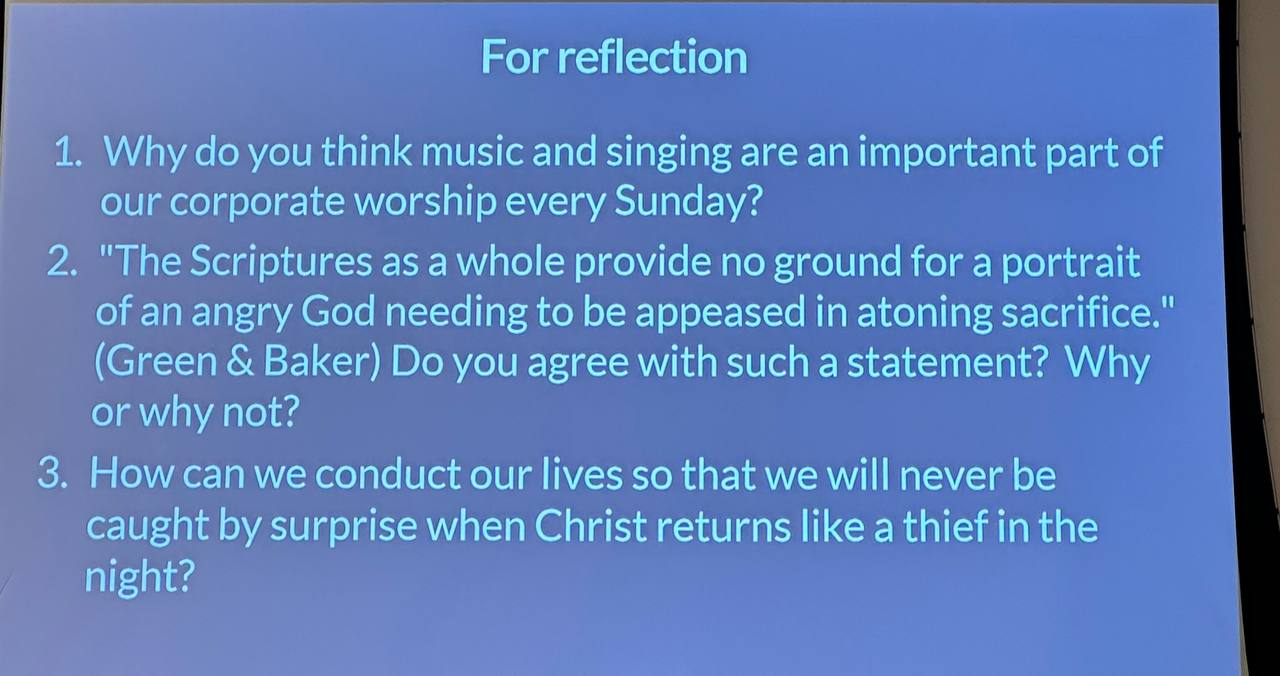
\includegraphics[width=0.8\textwidth, trim={0cm 0cm 0cm 0cm},clip]{Figures/marchSermon4Reflections.jpg}
  %   \includegraphics[width=0.8\textwidth, trim={0cm 0cm 0cm 0cm},clip]{example-image-a}
  %   \caption[]{Reflection questions for this sermon}
  %   \label{}
  % \end{figure}}
\end{itemize}